\section{Differential expression analysis}

\subsection{\Glspl{crna} associated with estrogen receptor expression}

\begin{figure}[H] \begin{tabular}{cc}
        \begin{subfigure}{0.5\textwidth} \centering

            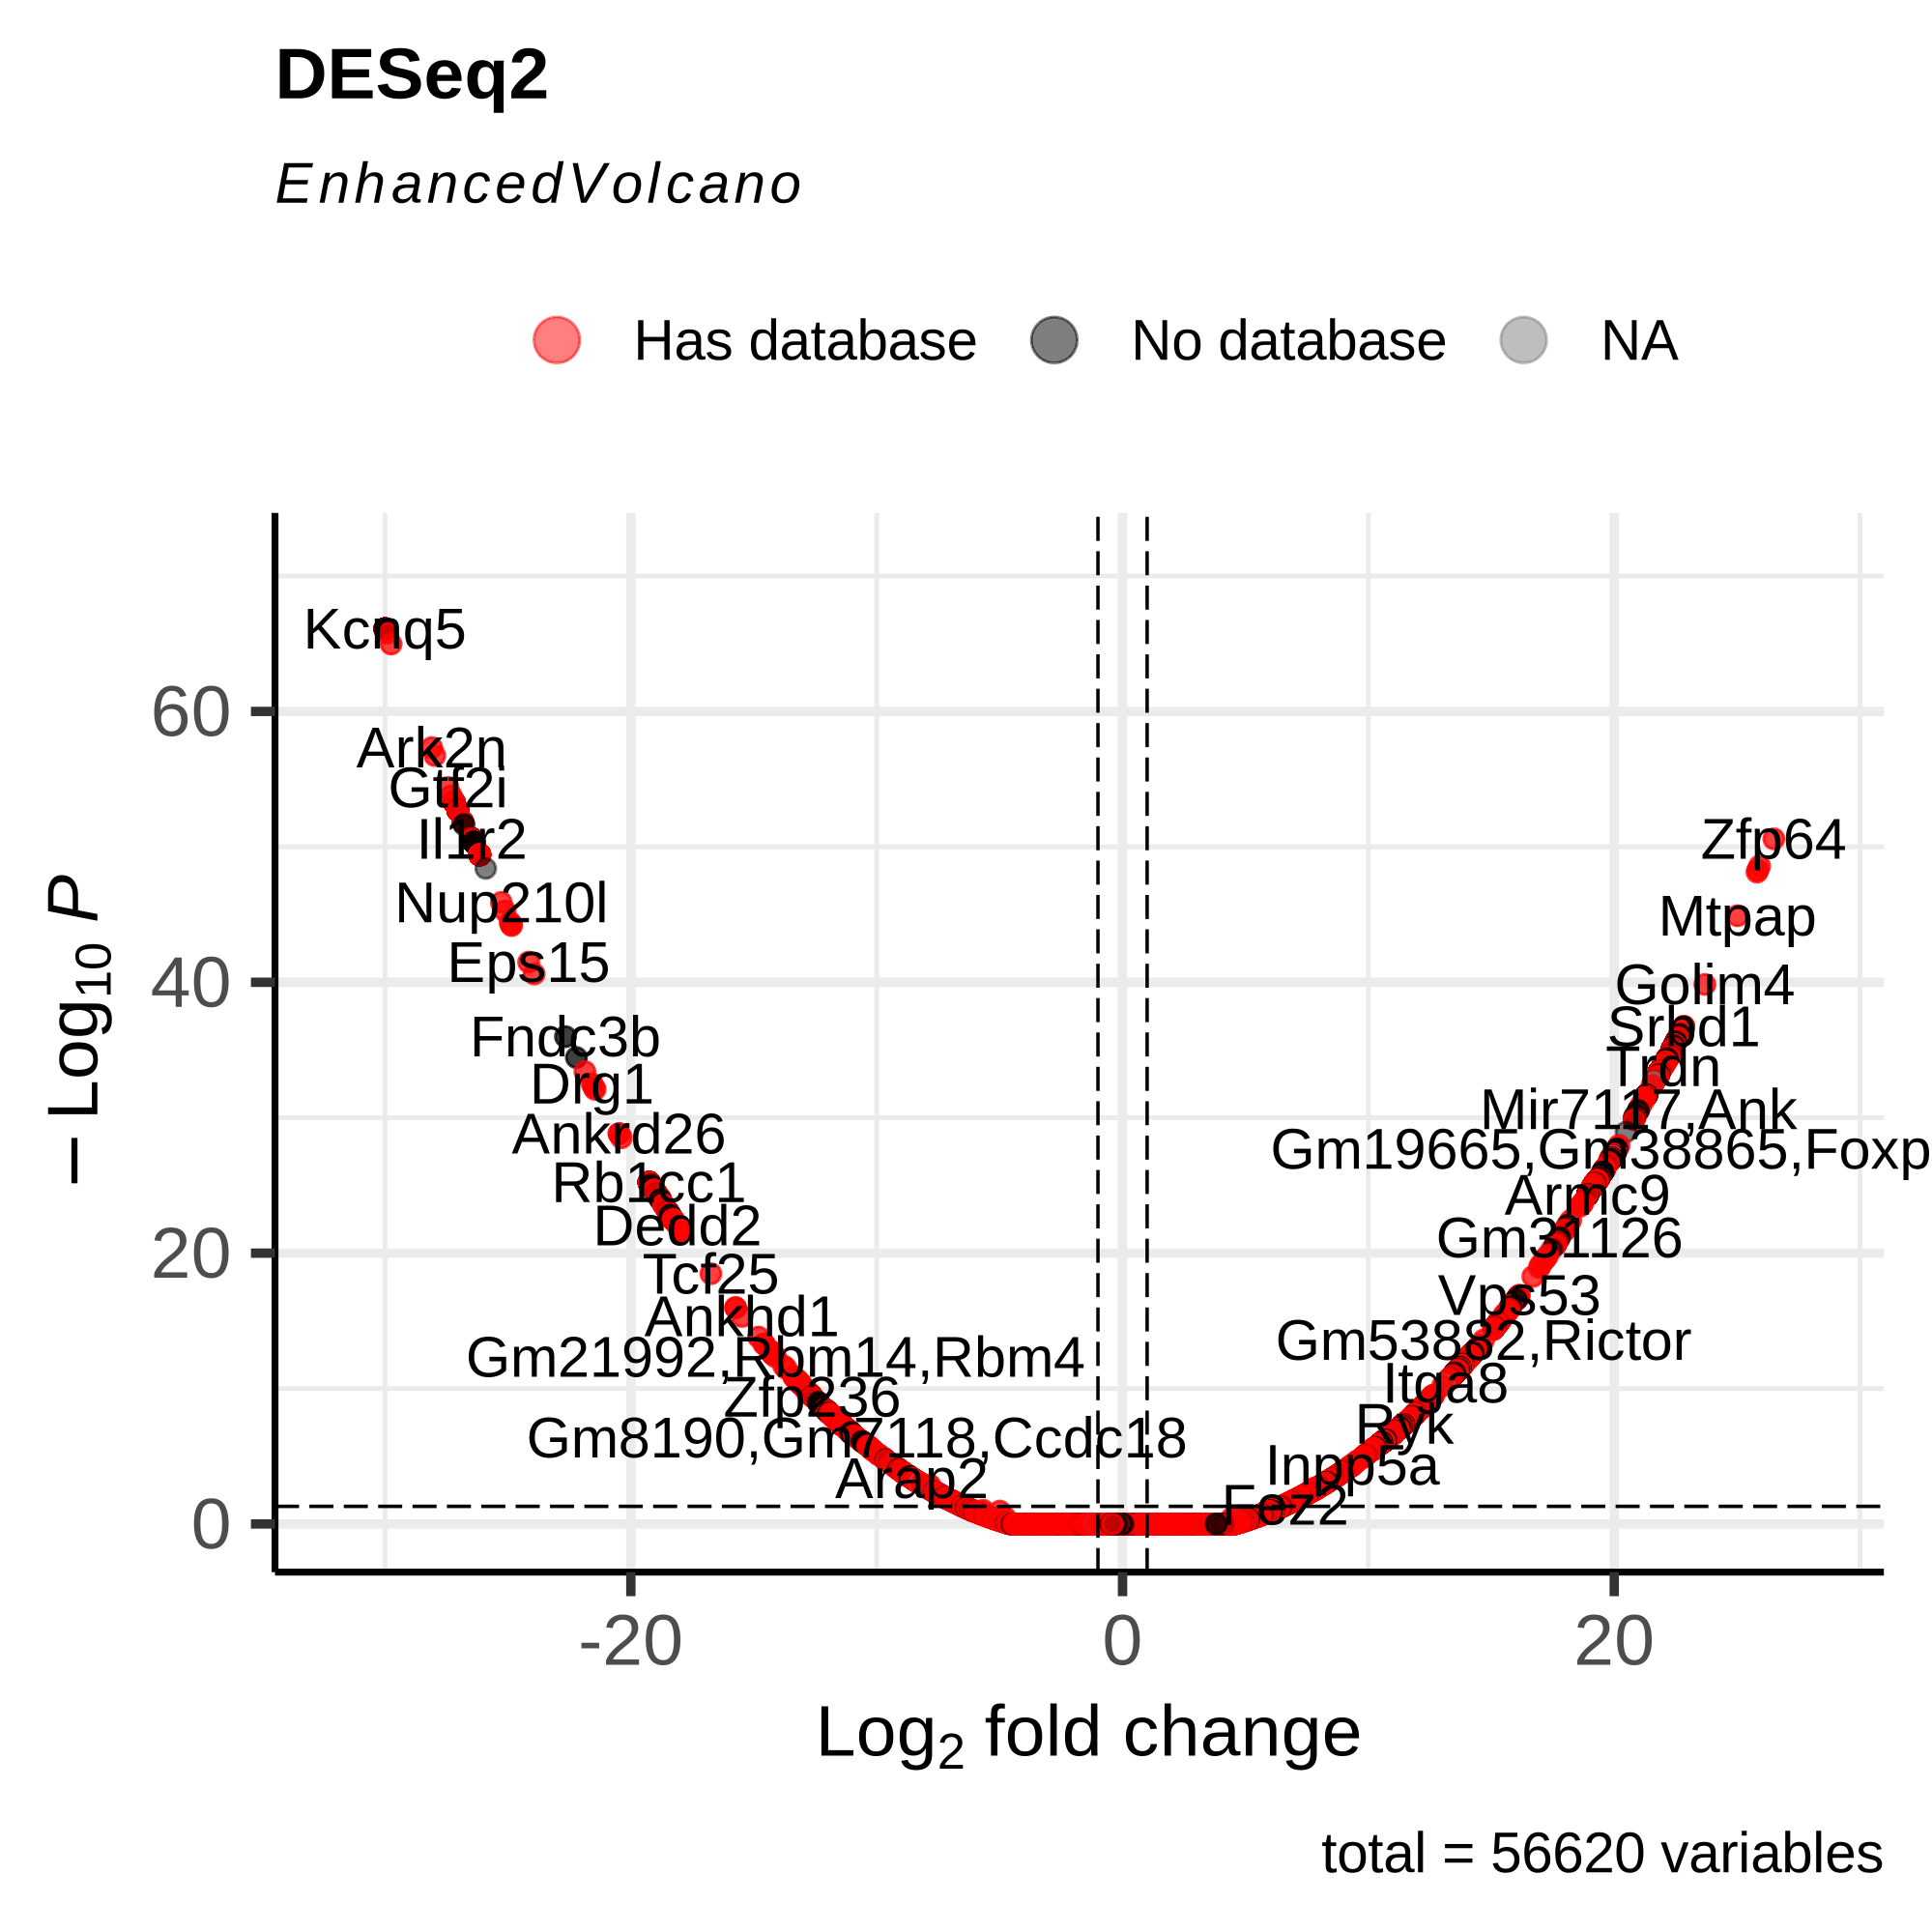
\includegraphics[width=\linewidth]{chapters/4_results_and_discussion/figures/dea/deseq2/esr1/volcano.png}
            \caption{Hello world!
            }
            \label{fig:esr1_volcano}
        \end{subfigure}
        \begin{subfigure}{0.5\textwidth}
            \centering

            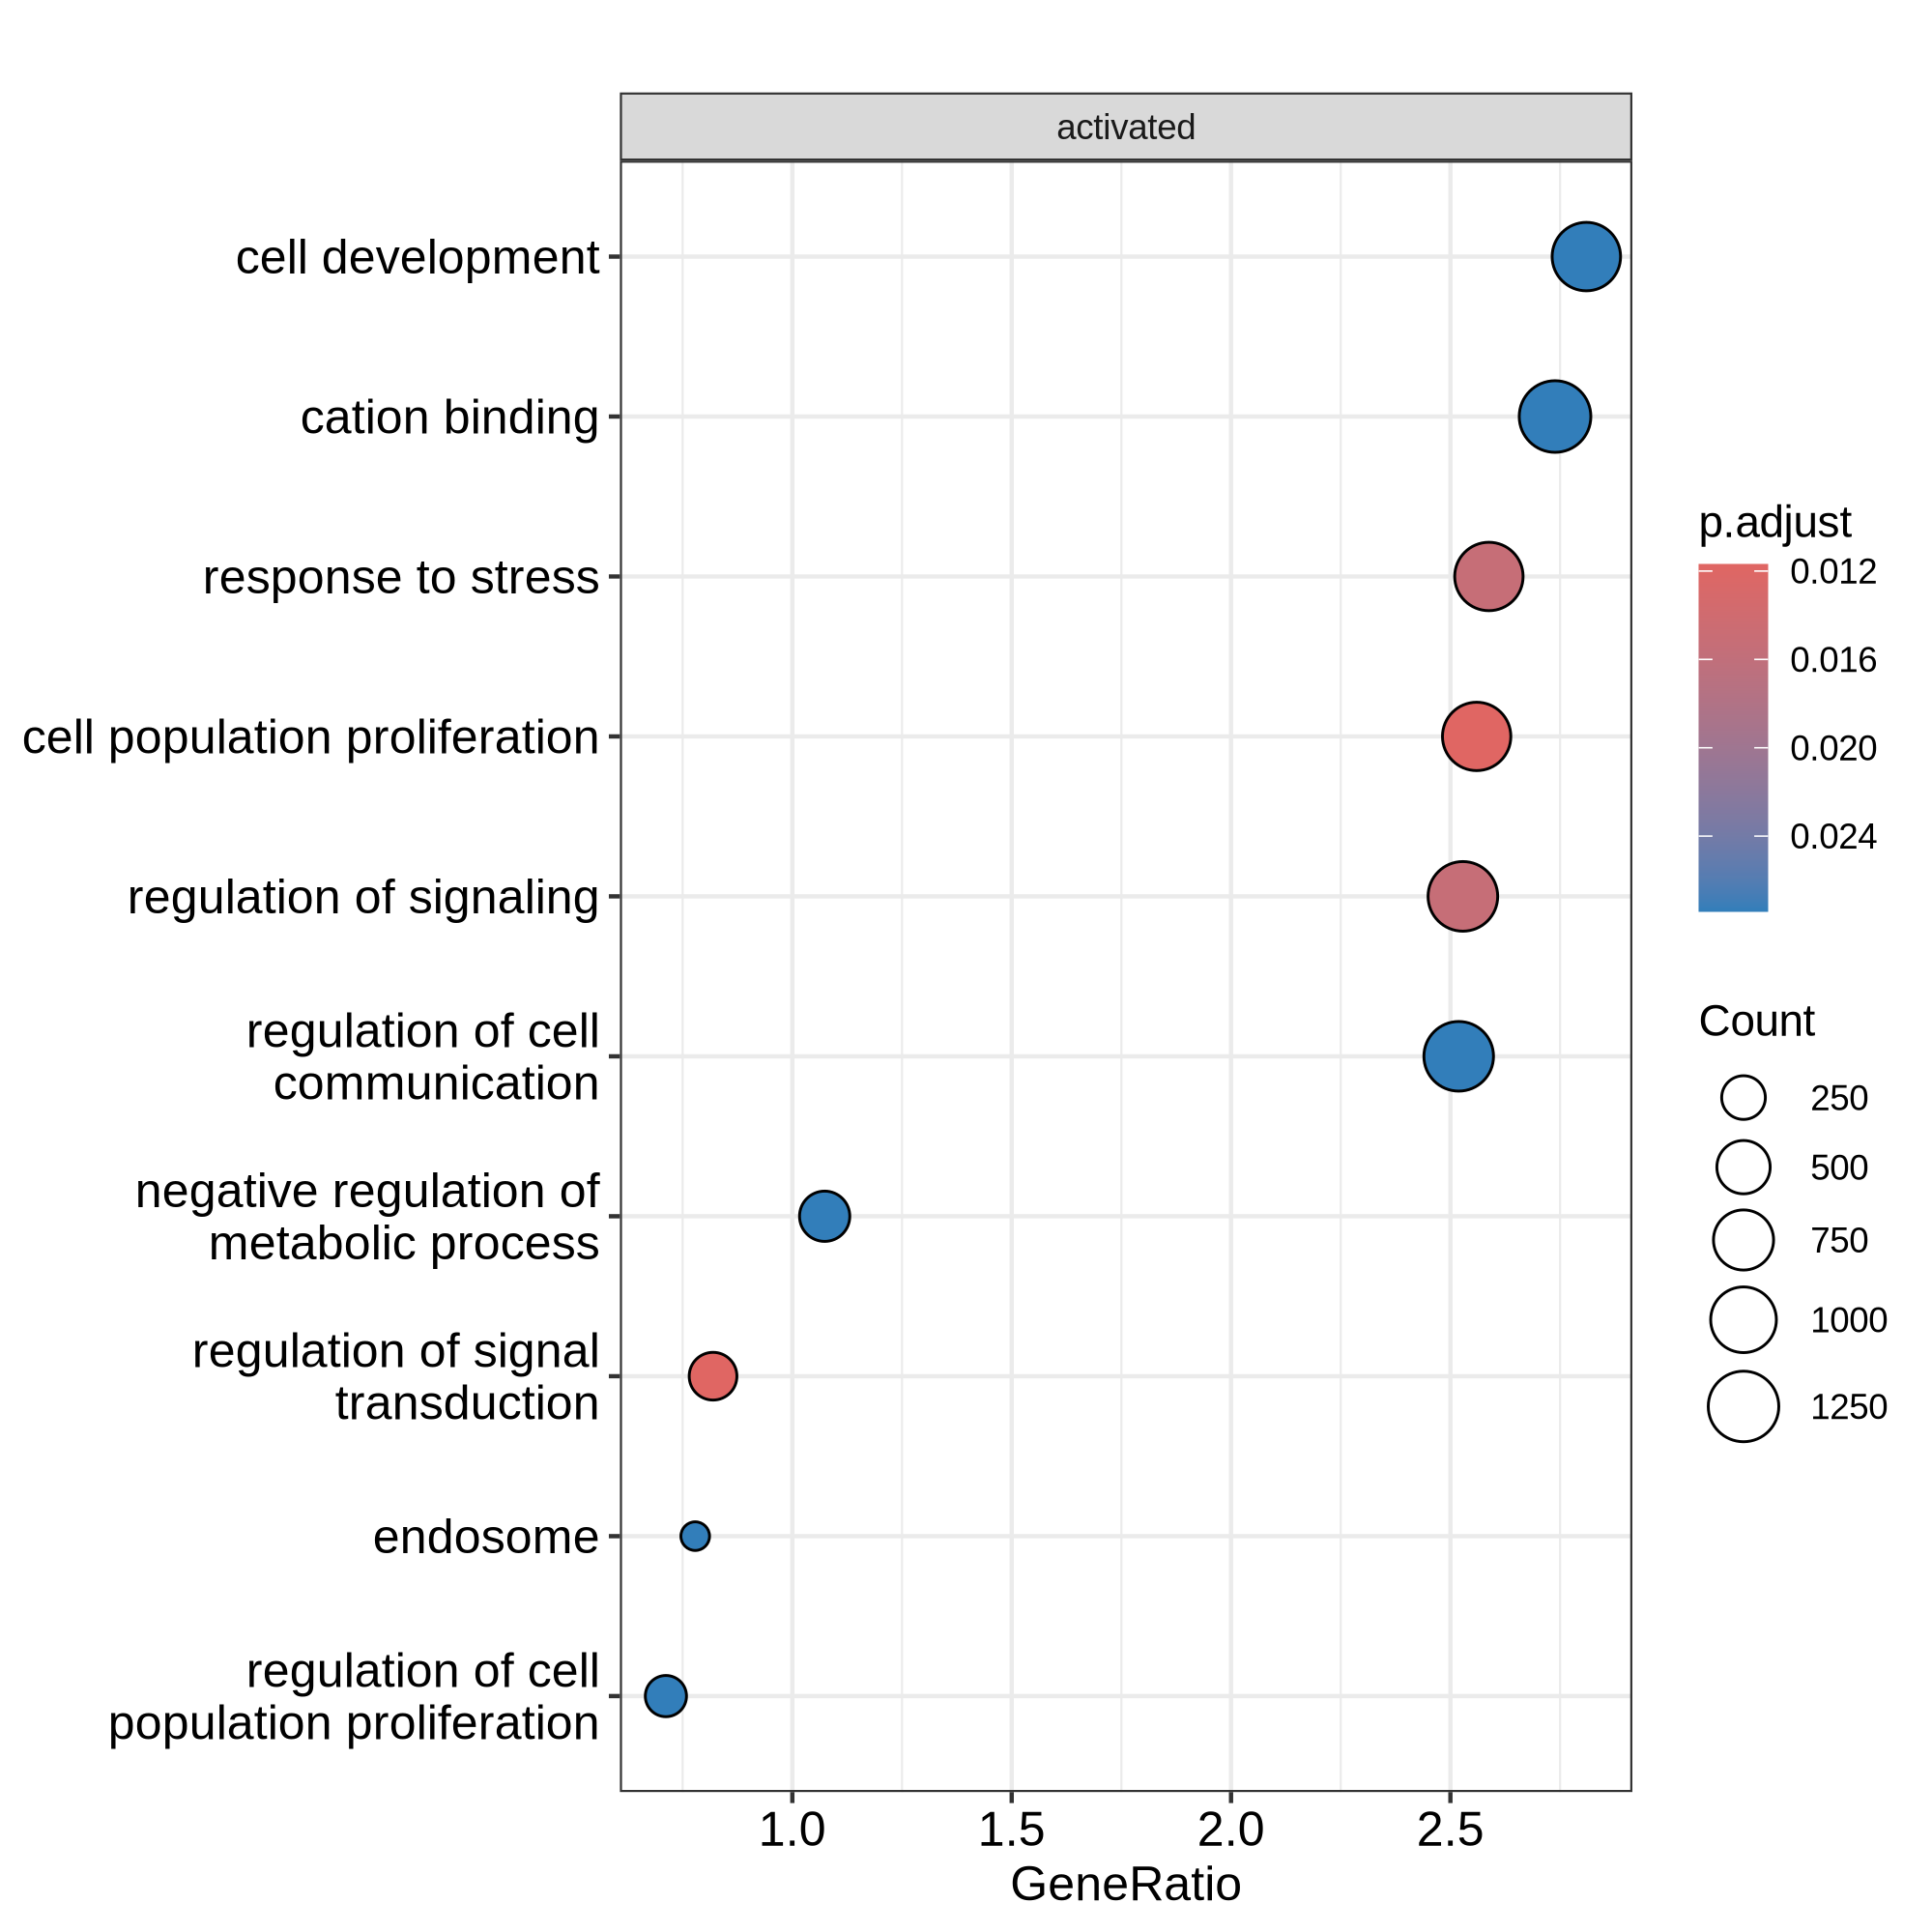
\includegraphics[width=\linewidth]{chapters/4_results_and_discussion/figures/dea/deseq2/esr1/dot.png}
            \caption{Hello world!
            }
            \label{fig:esr1_go_terms}
        \end{subfigure} &

    \end{tabular}
    \caption{As \cref{fig:db_pie} shows, while there is a large fraction of
        \glspl{crna} without any
        database match, more than 50\% of detected \glspl{crna} at least one
        hit.
        As shown in \cref{fig:db_upset}, most hits are from \gls{circatlas}, which is
        most likely due to the fact that it is the largest database.
        While both \gls{cb-m} and \gls{cb-h} have some exclusive hits, the majority of
        their hits are shared with \gls{circatlas}.
    }
    \label{fig:dea_esr1}
\end{figure}

\subsection{\Glspl{crna} associated with tamoxifen induction}

\begin{figure}[H] \begin{tabular}{cc}
        \begin{subfigure}{0.5\textwidth} \centering

            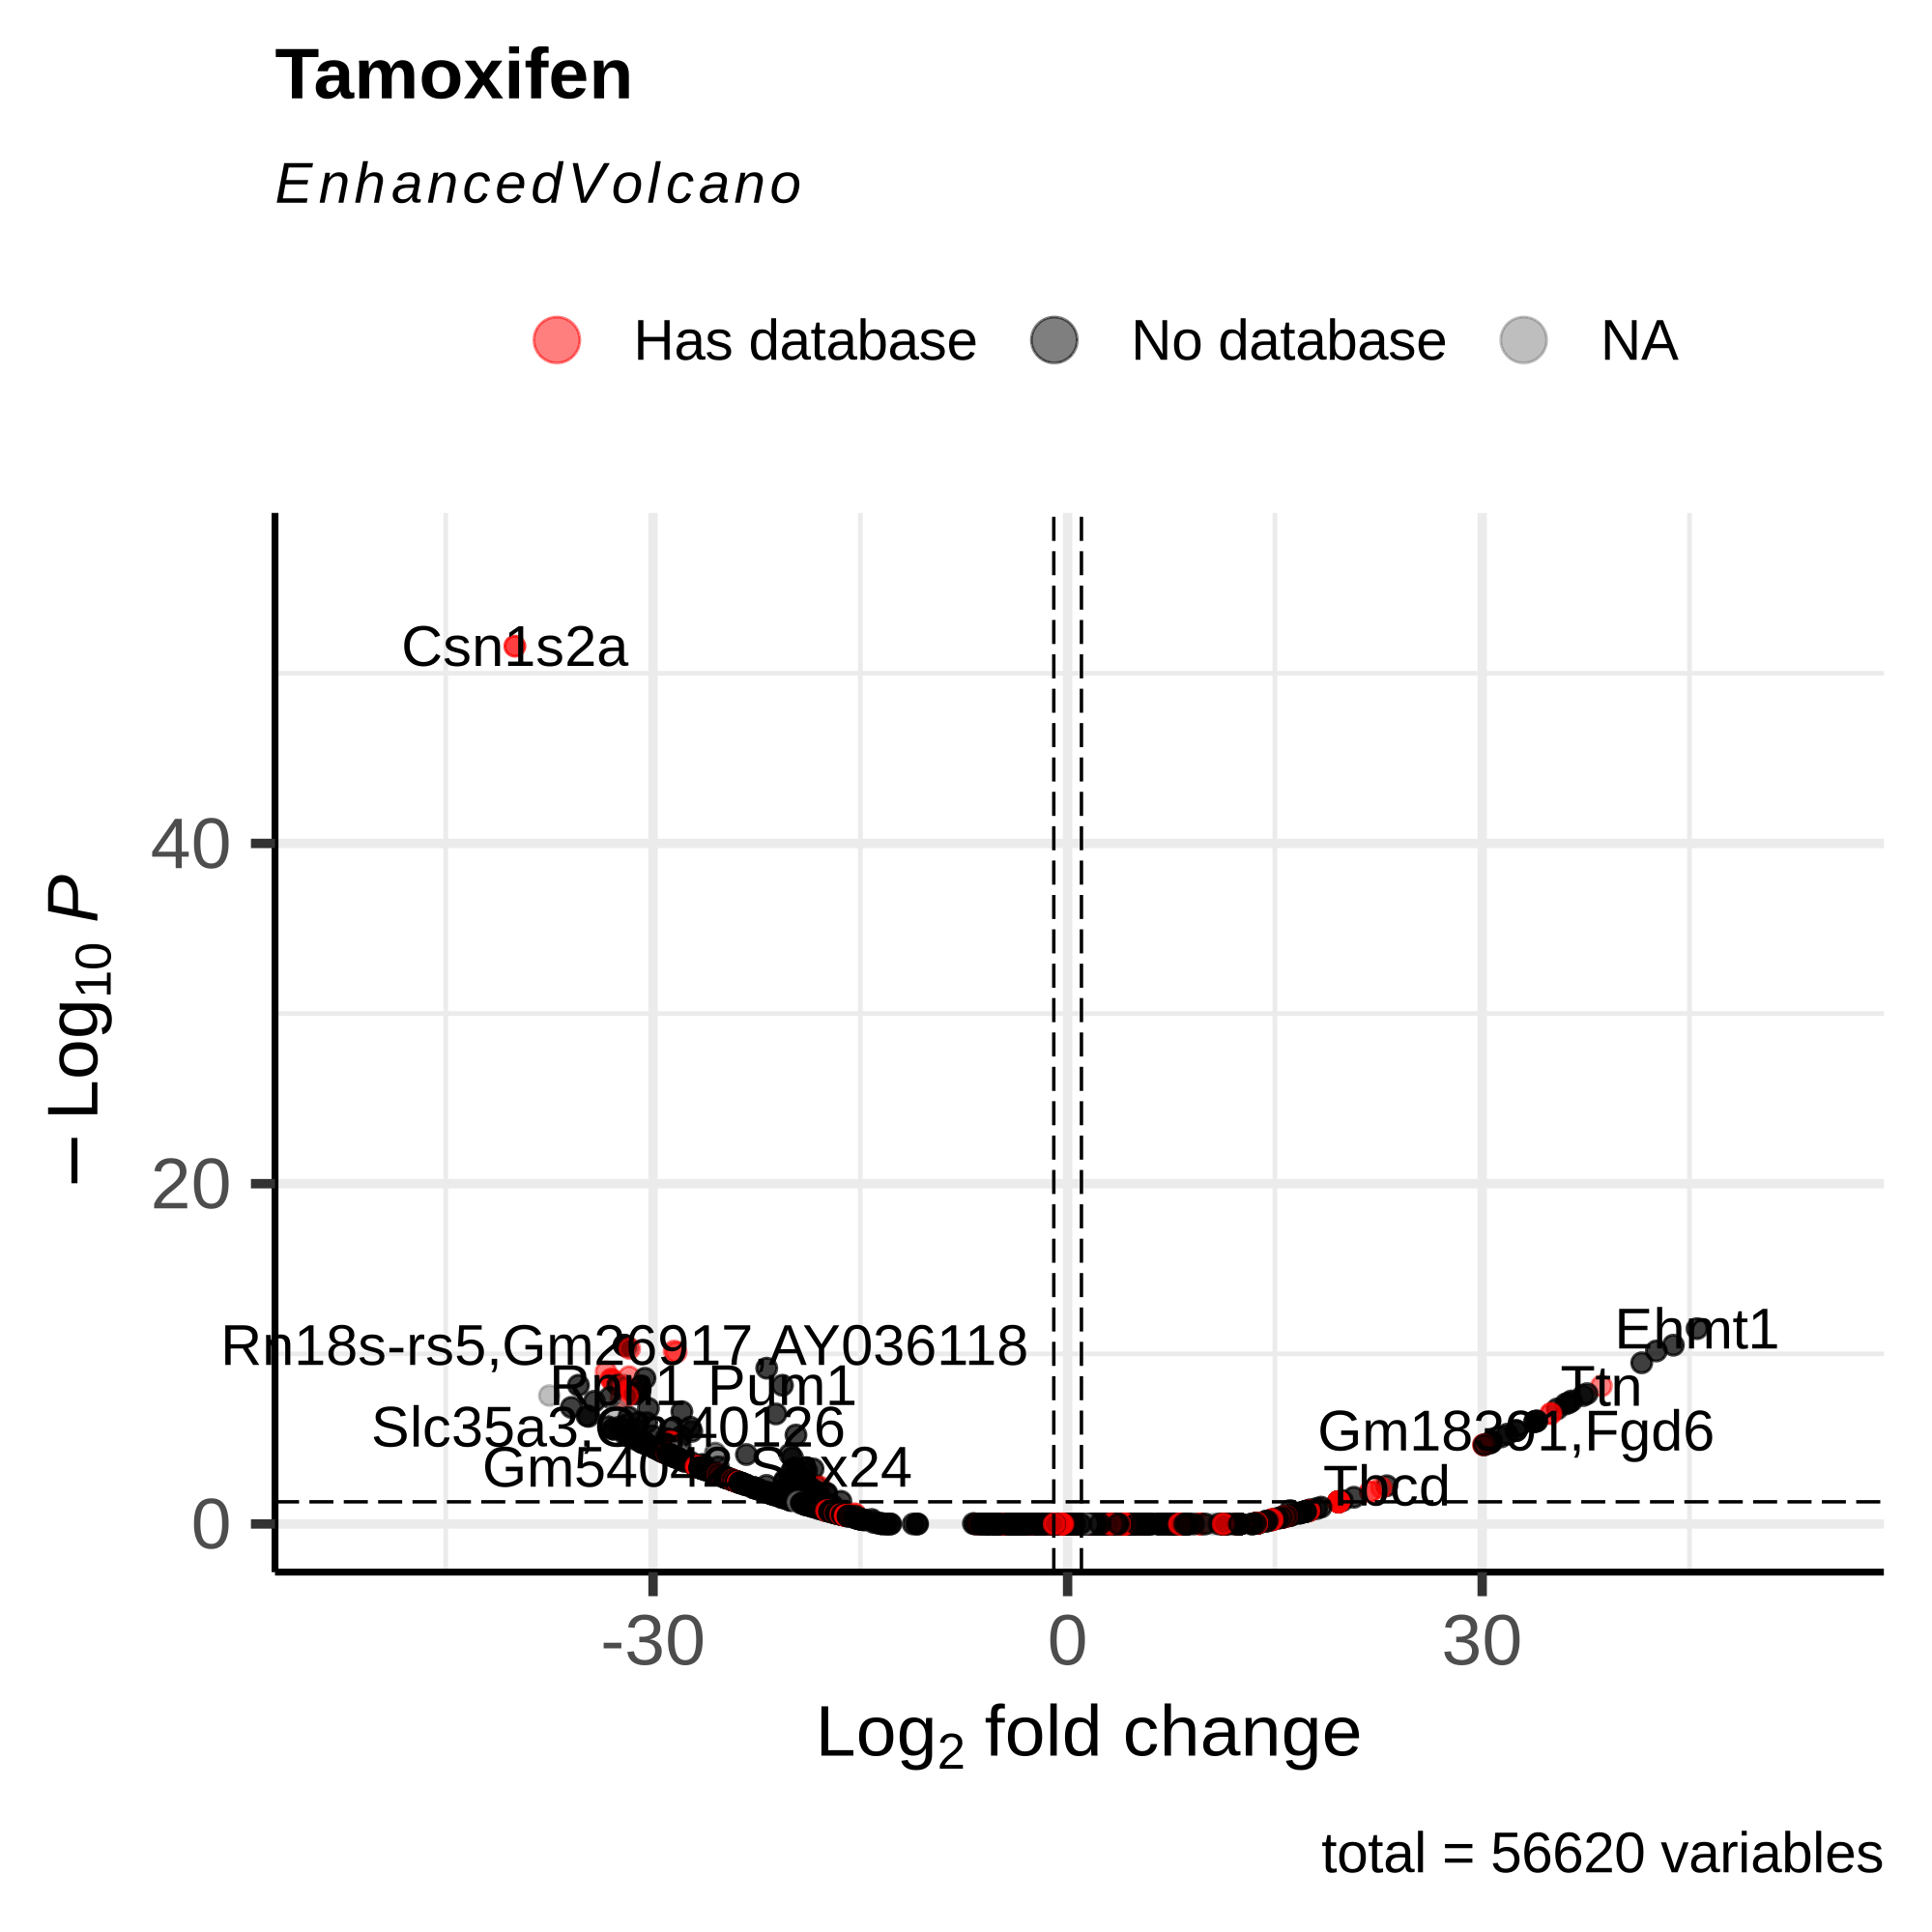
\includegraphics[width=\linewidth]{chapters/4_results_and_discussion/figures/dea/deseq2/tamoxifen/volcano.png}
            \caption{Fractions of \glspl{crna} supported by
                different numbers of databases}
            \label{fig:tamoxifen_volcano_deseq2}
        \end{subfigure}
        \begin{subfigure}{0.5\textwidth}
            \centering

            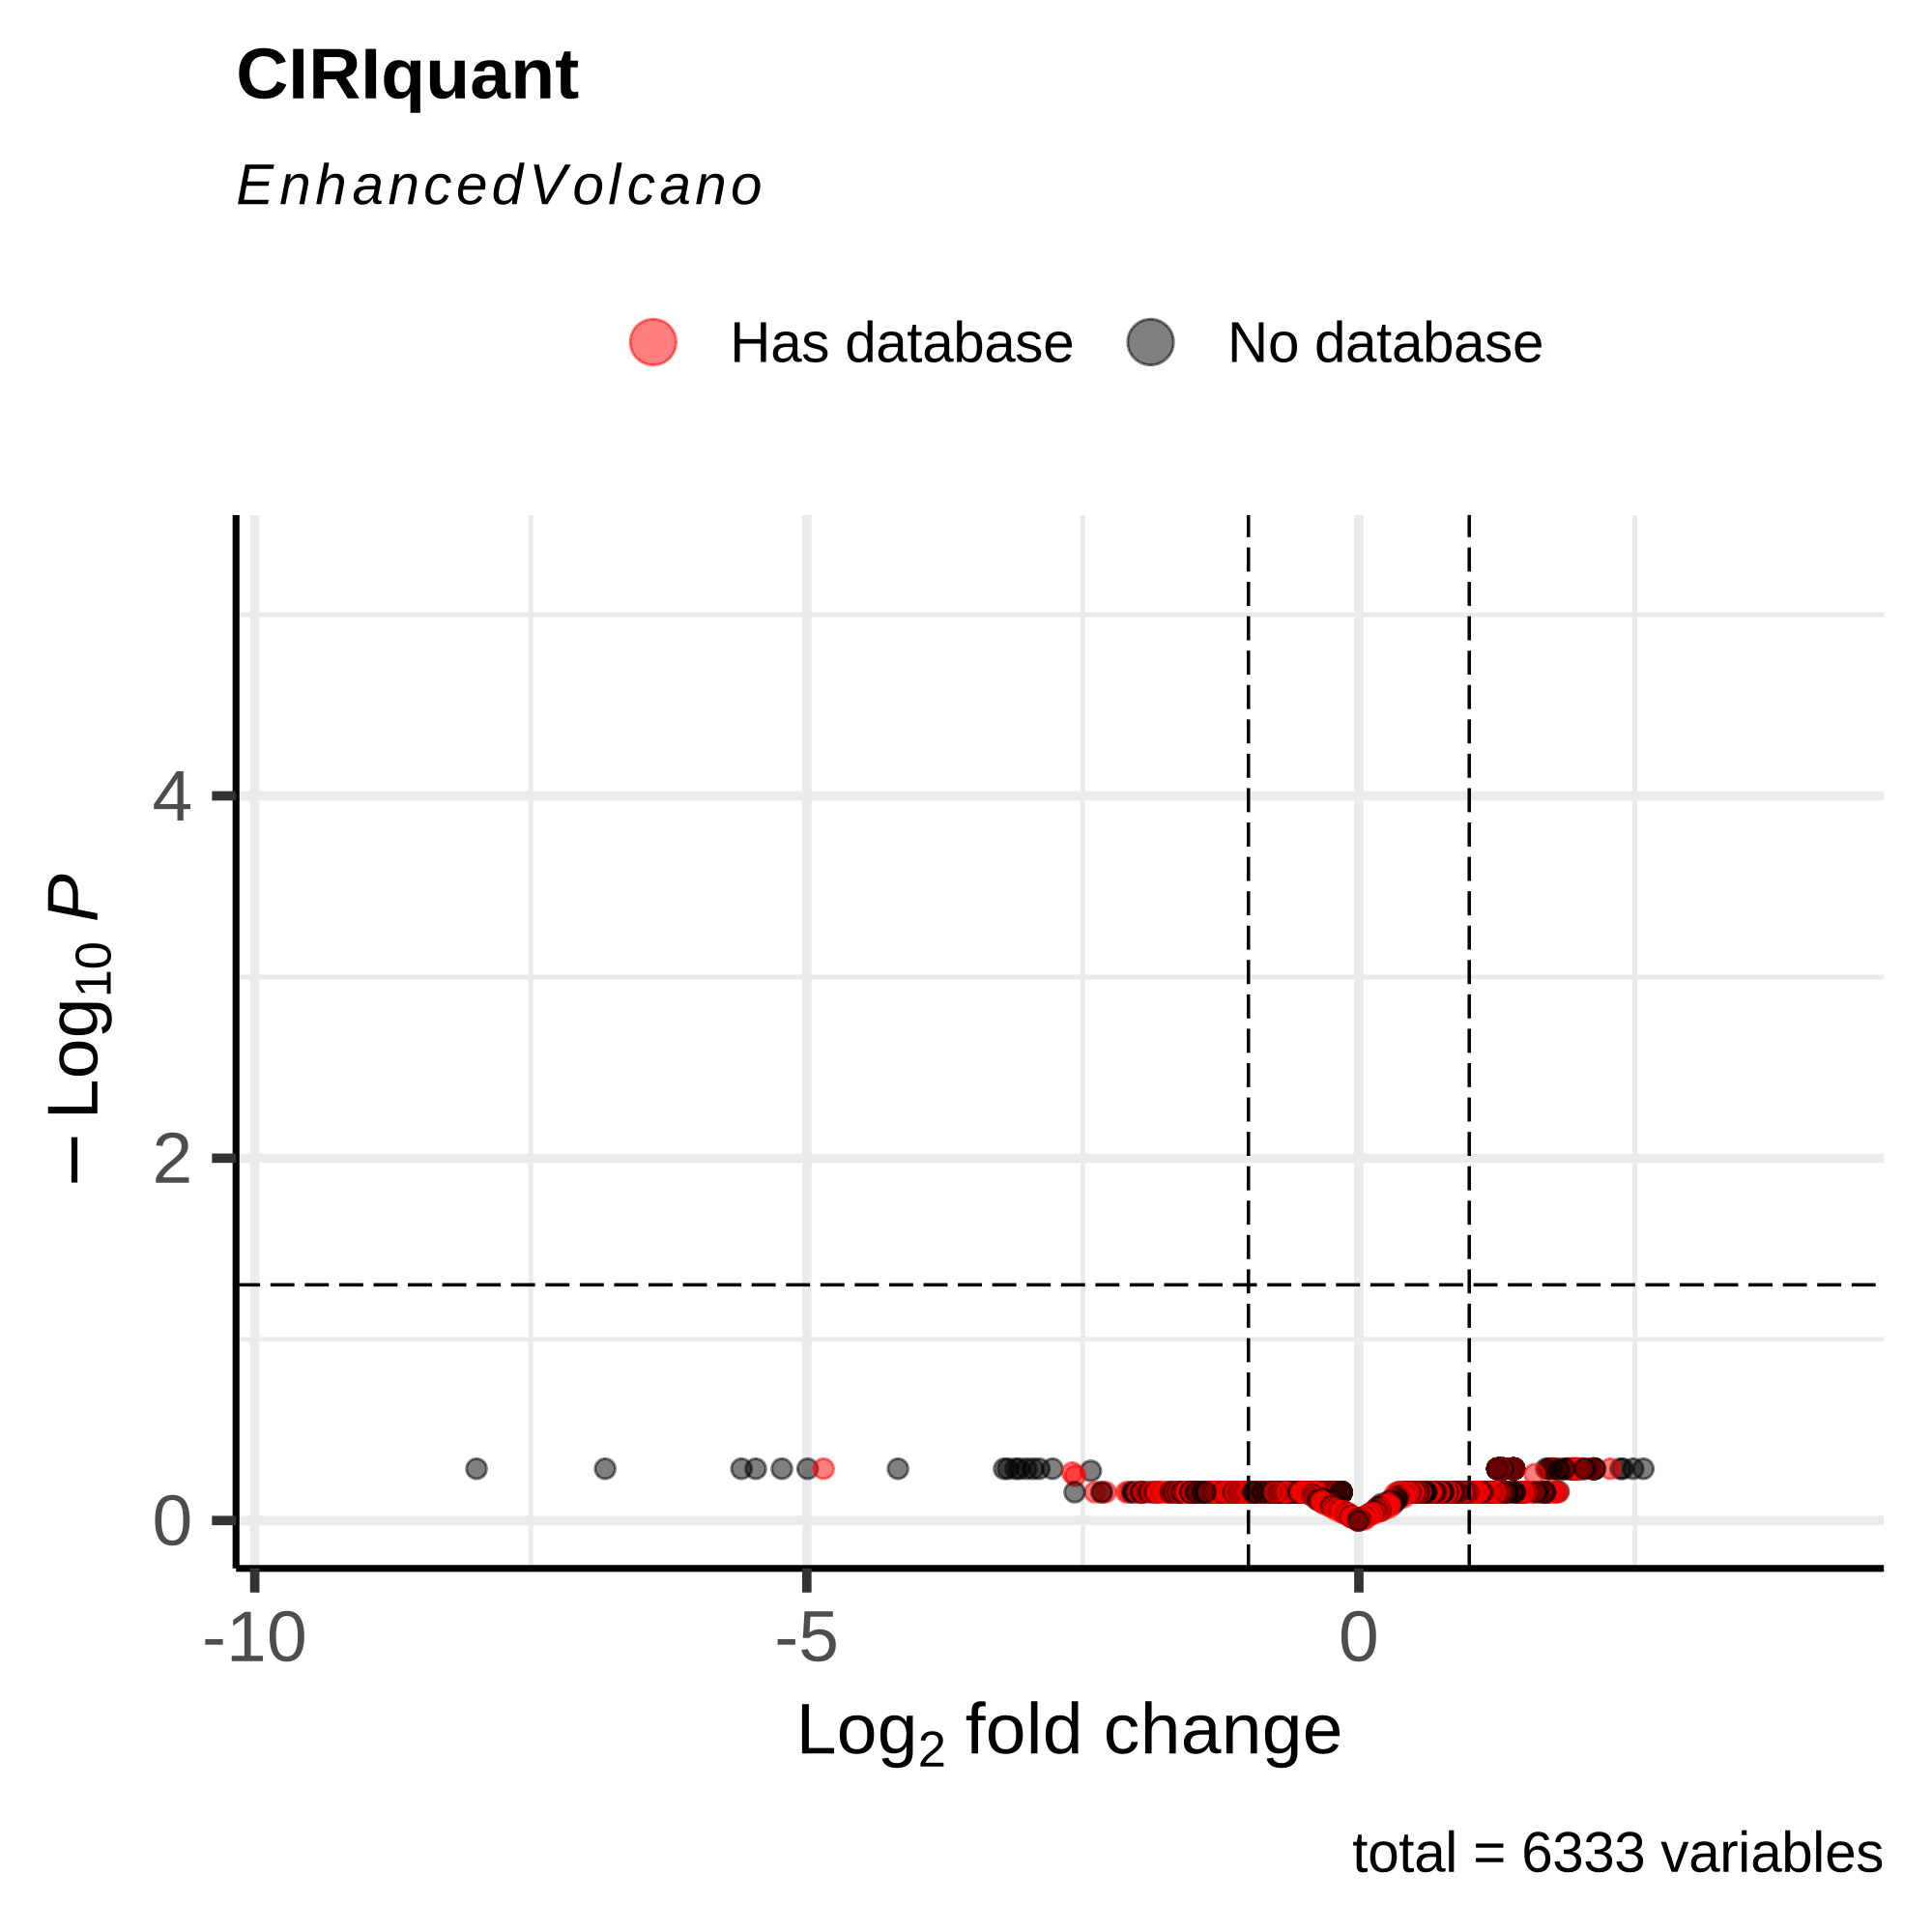
\includegraphics[width=\linewidth]{chapters/4_results_and_discussion/figures/dea/ciriquant/tamoxifen/volcano.png}
            \caption{Agreement between detected
                \glspl{bsj} and databases}
            \label{fig:tamoxifen_volcano_ciriquant}
        \end{subfigure} &

    \end{tabular}
    \caption{As \cref{fig:db_pie} shows, while there is a large fraction of
        \glspl{crna} without any
        database match, more than 50\% of detected \glspl{crna} at least one
        hit.
        As shown in \cref{fig:db_upset}, most hits are from \gls{circatlas}, which is
        most likely due to the fact that it is the largest database.
        While both \gls{cb-m} and \gls{cb-h} have some exclusive hits, the majority of
        their hits are shared with \gls{circatlas}.
    }
    \label{fig:tamoxifen_volcano}
\end{figure}

\subsection{\Glspl{crna} associated with letrozole induction}

\begin{figure}[H] \begin{tabular}{cc}
        \begin{subfigure}{0.5\textwidth} \centering

            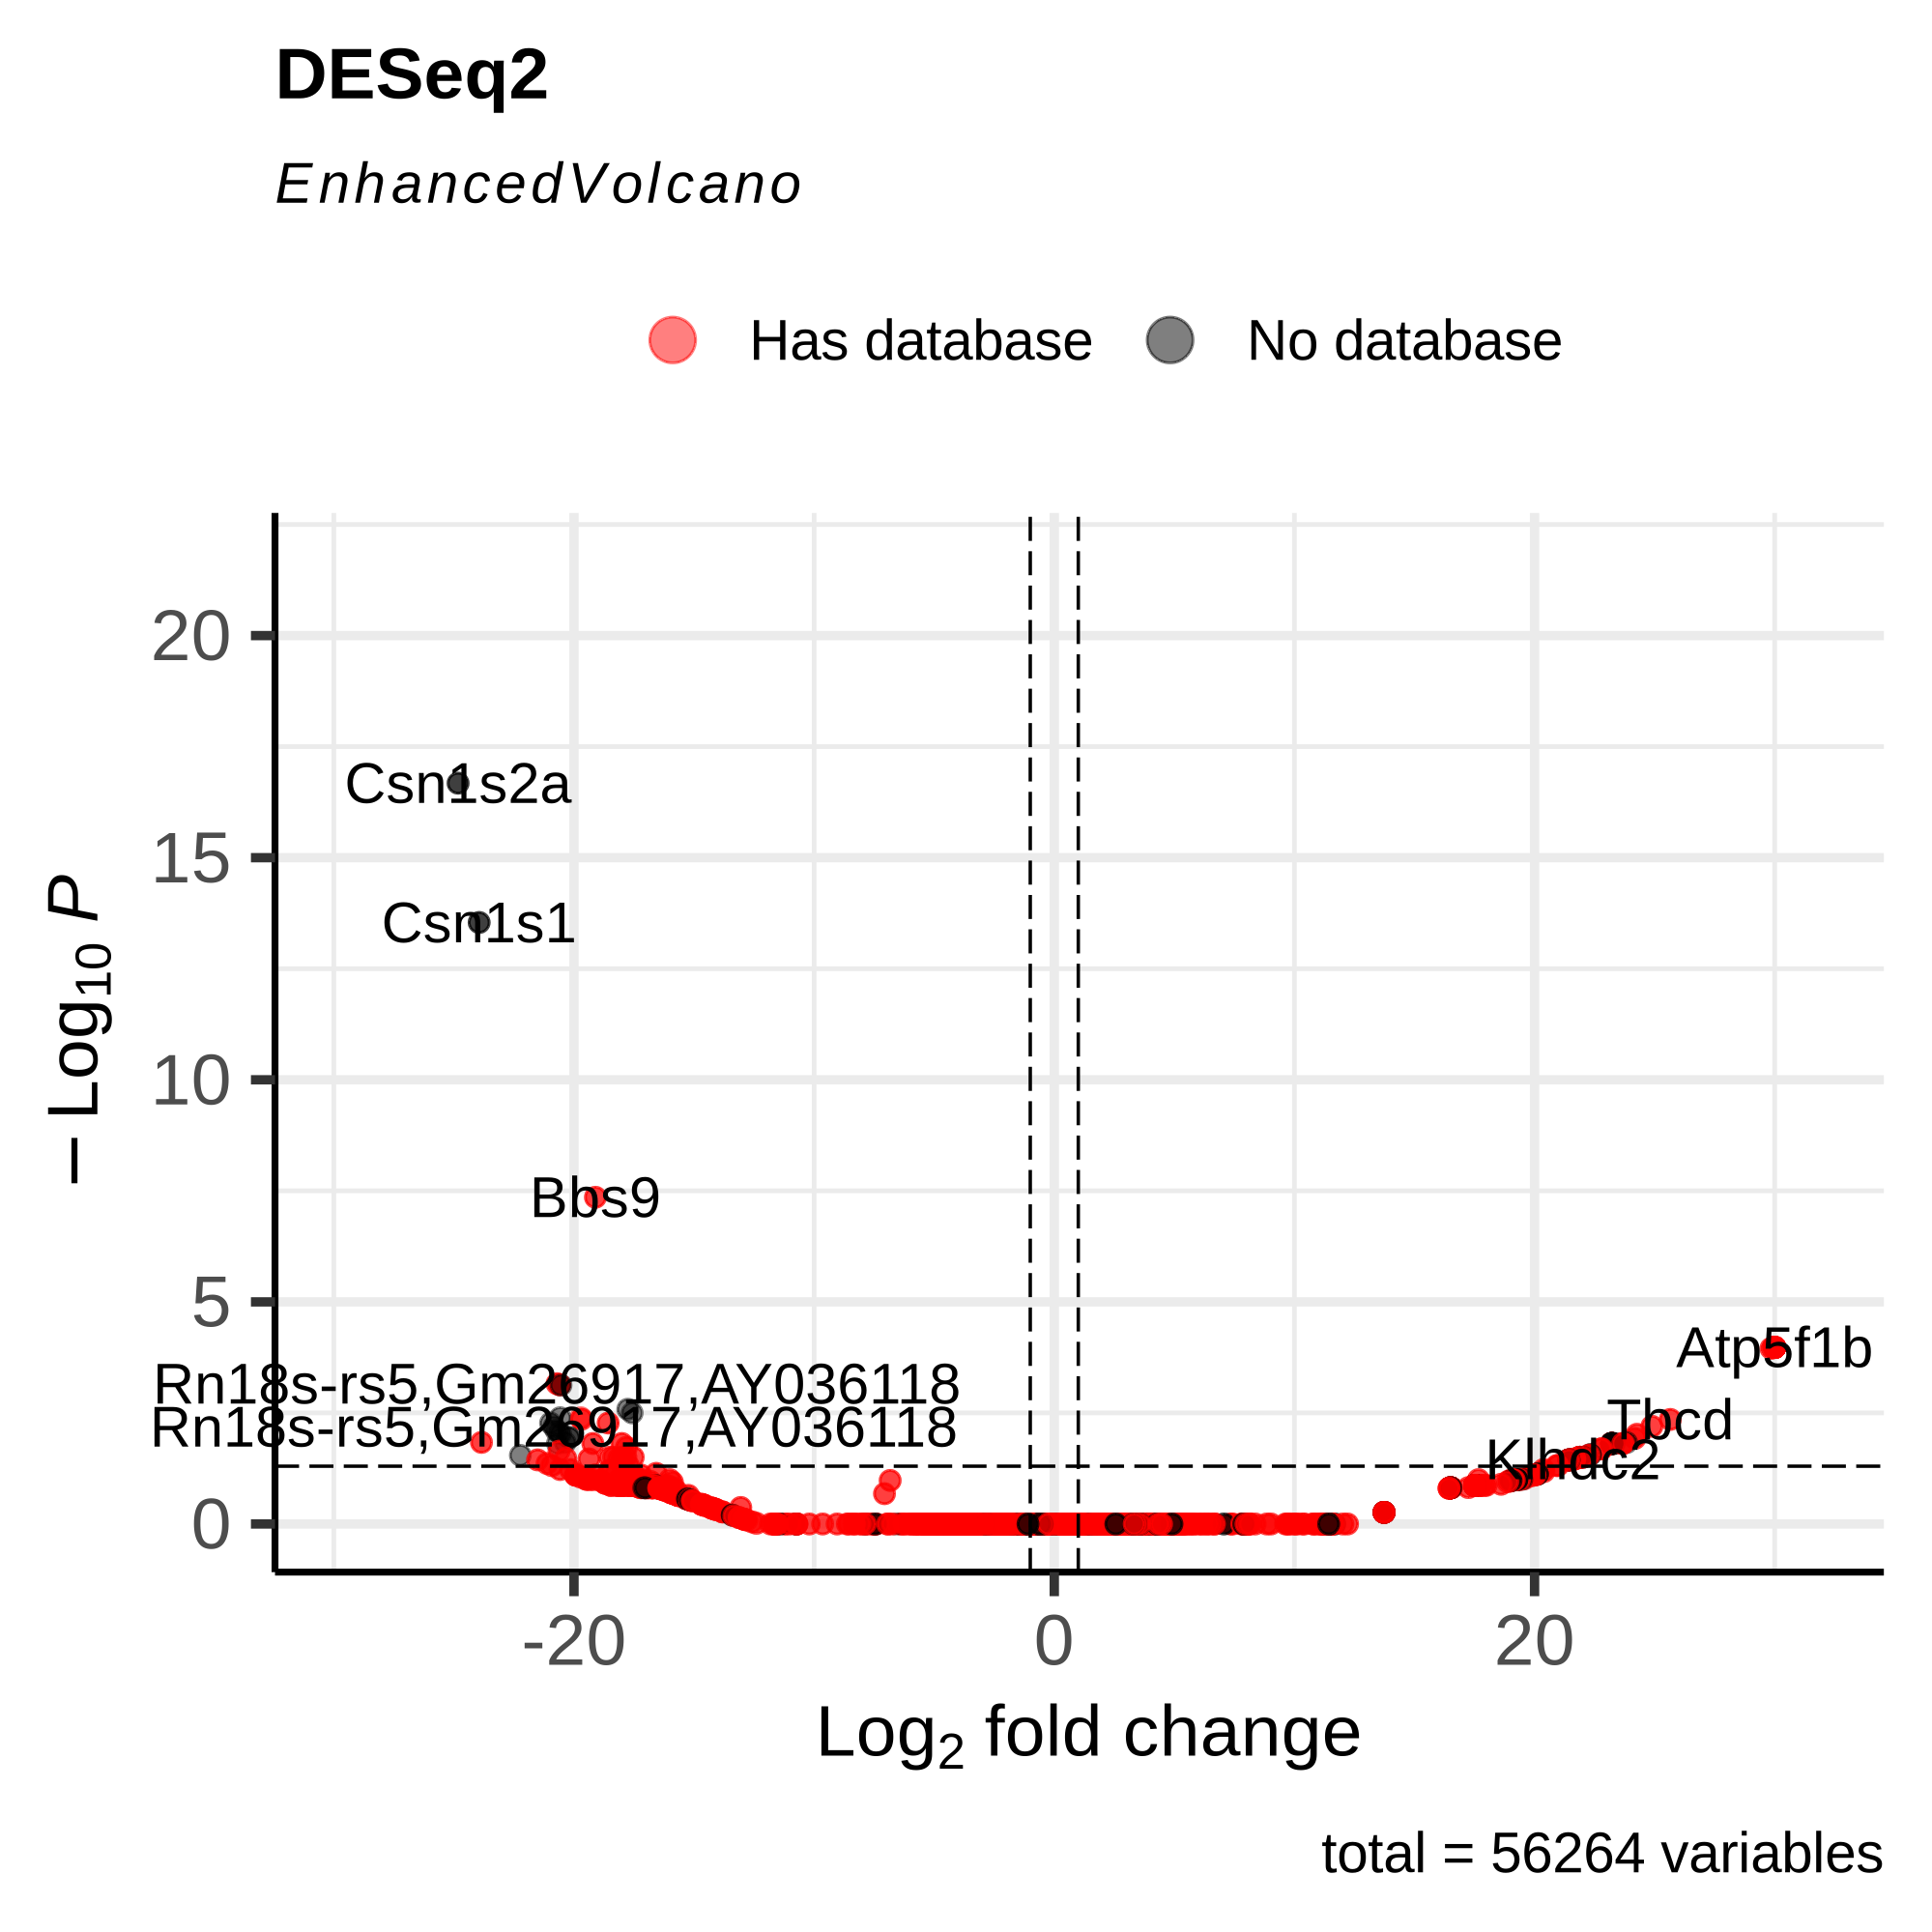
\includegraphics[width=\linewidth]{chapters/4_results_and_discussion/figures/dea/deseq2/letrozole/volcano.png}
            \caption{Fractions of \glspl{crna} supported by
                different numbers of databases}
            \label{fig:letrozole_volcano_deseq2}
        \end{subfigure}
        \begin{subfigure}{0.5\textwidth}
            \centering

            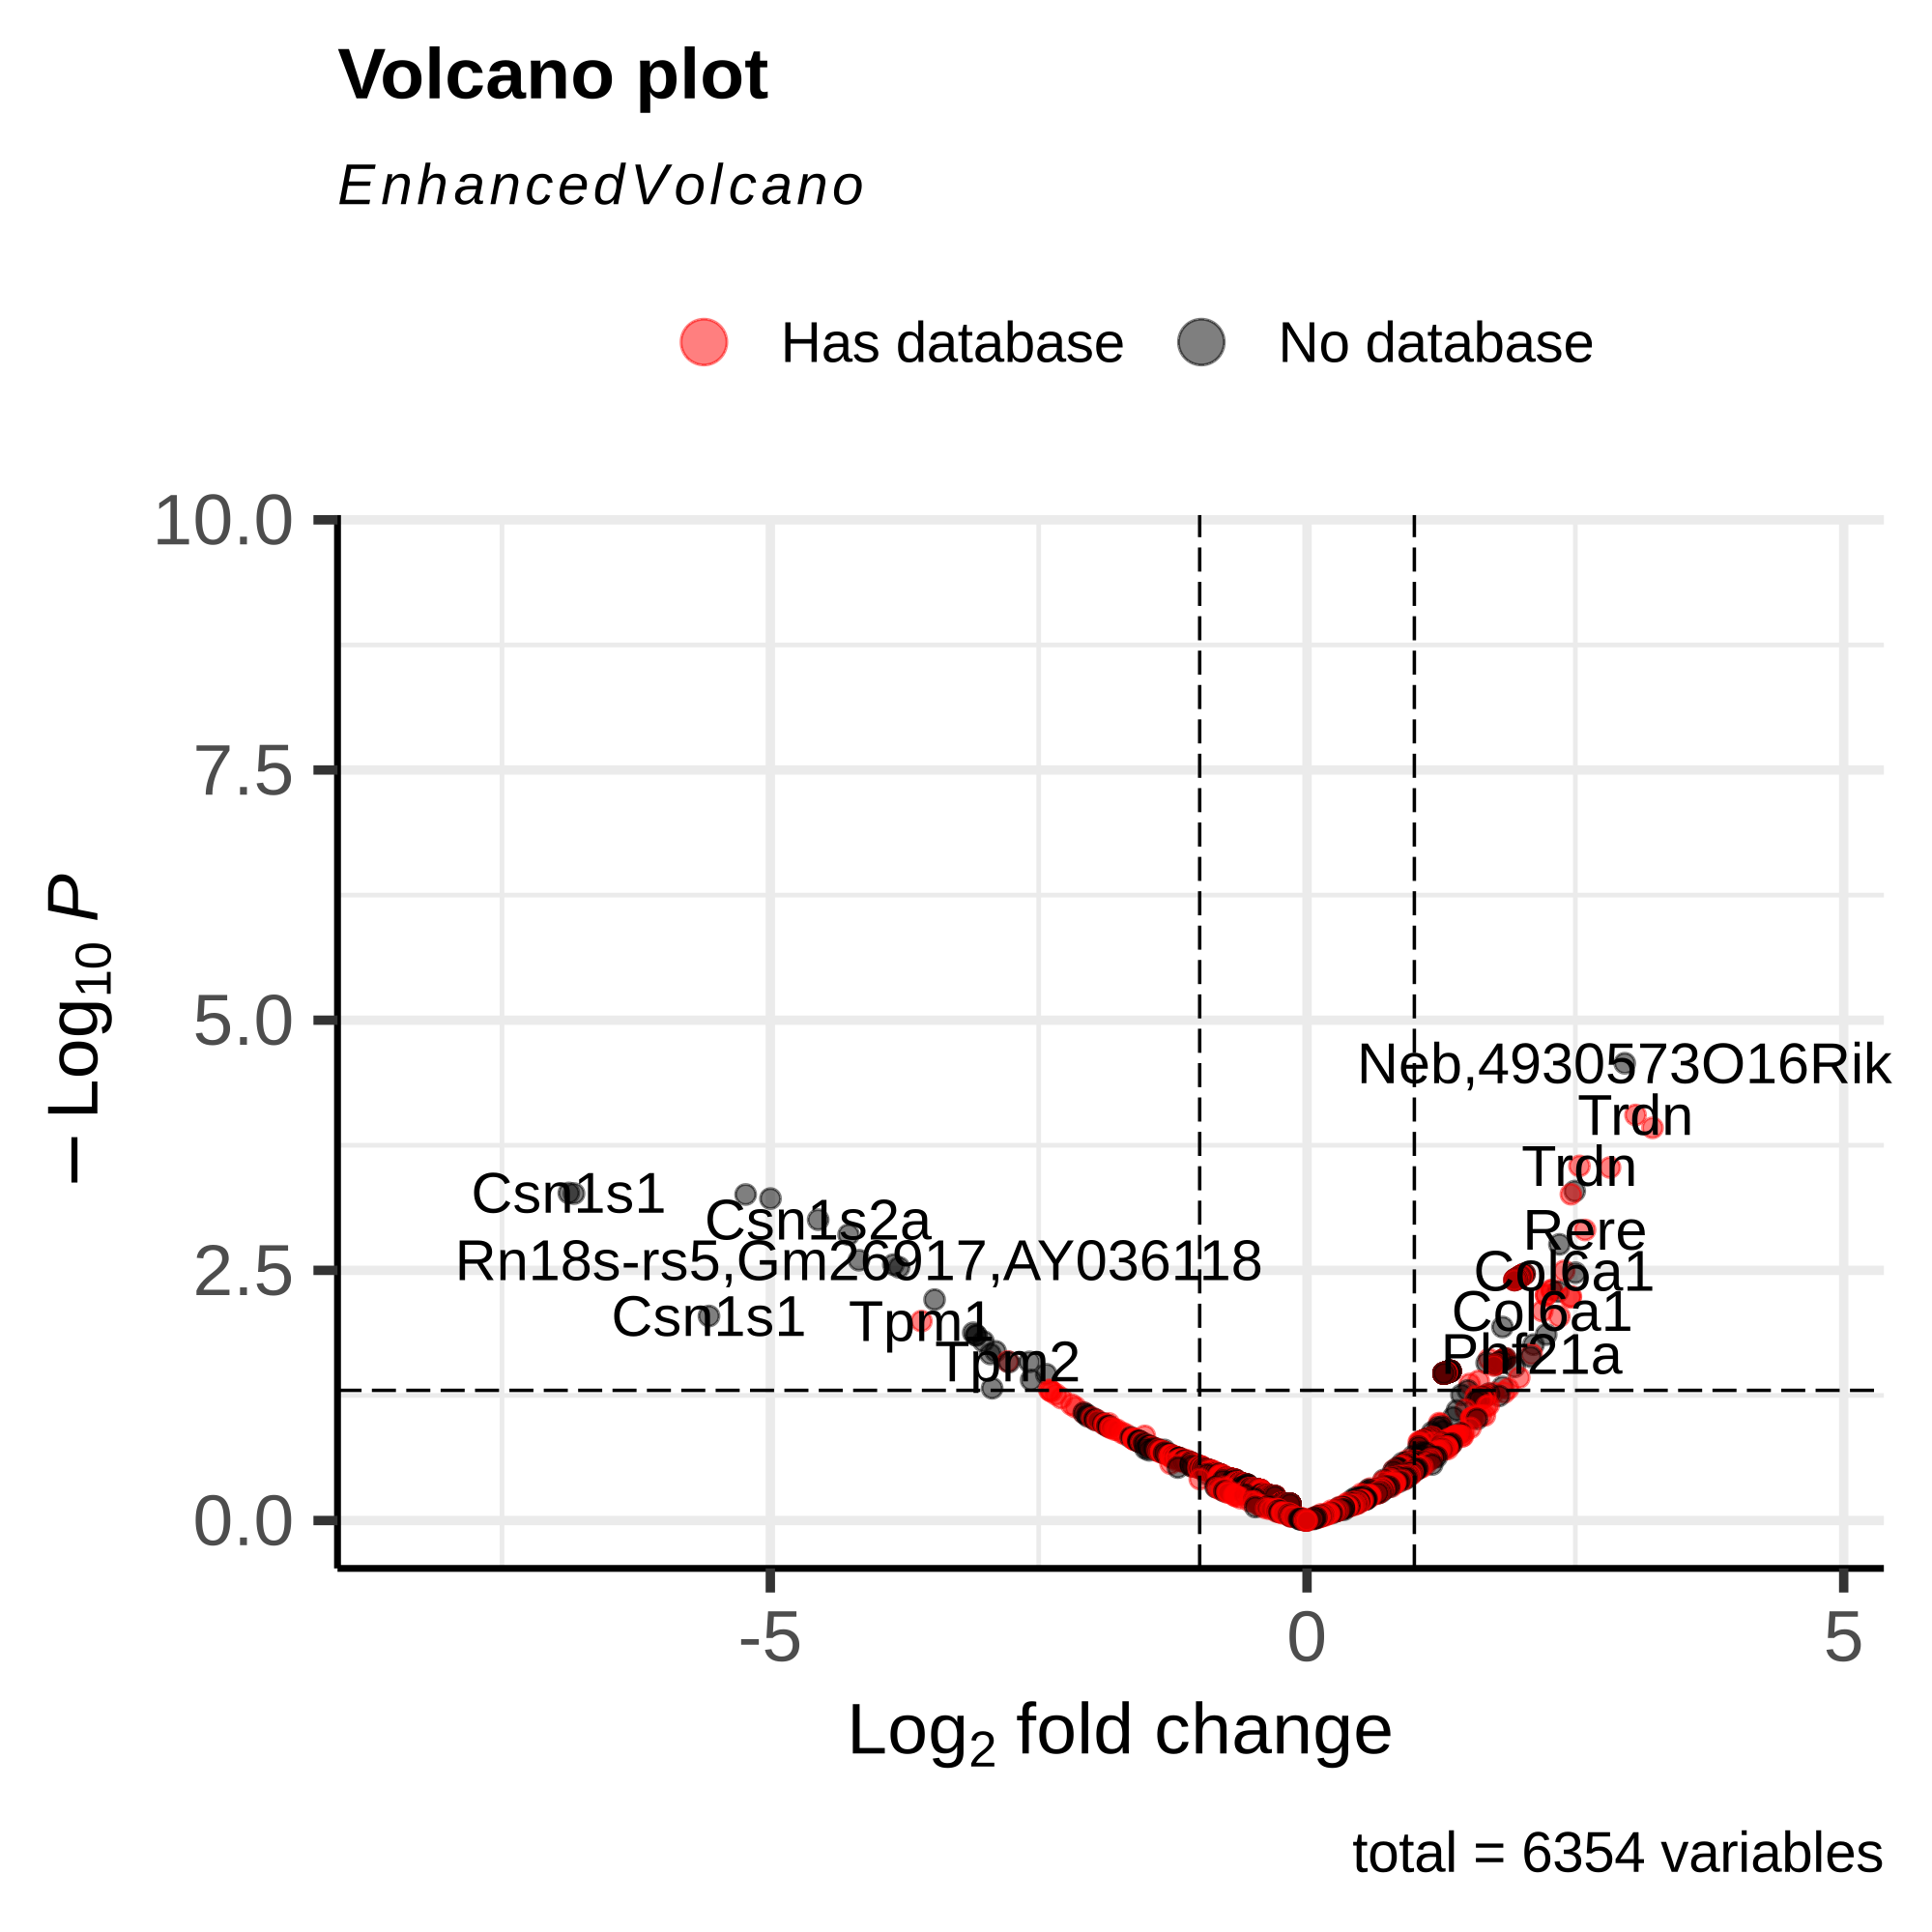
\includegraphics[width=\linewidth]{chapters/4_results_and_discussion/figures/dea/ciriquant/letrozole/volcano.png}
            \caption{Agreement between detected
                \glspl{bsj} and databases}
            \label{fig:letrozole_volcano_ciriquant}
        \end{subfigure} &

    \end{tabular}
    \caption{As \cref{fig:db_pie} shows, while there is a large fraction of
        \glspl{crna} without any
        database match, more than 50\% of detected \glspl{crna} at least one
        hit.
        As shown in \cref{fig:db_upset}, most hits are from \gls{circatlas}, which is
        most likely due to the fact that it is the largest database.
        While both \gls{cb-m} and \gls{cb-h} have some exclusive hits, the majority of
        their hits are shared with \gls{circatlas}.
    }
    \label{fig:letrozole_volcano}
\end{figure}

\subsection{Known \glsfmtshortpl{snp} located in differentially expressed
    \glsfmtshortpl{crna}}
